% !TEX root = ../thesis.tex


\chapter{Results and Evaluation}
\label{cha:dmd_results}
To test the correction algorithm(s), a pattern with full brightness and a black square in the centre is used, similar to what the experiment uses to make the box potential (Sec.~\ref{sec:dmd_experimental_setup}). The general goal is then to make the centre as flat as possible. We want to know how the correction handles aberrations in the dark centre. To do this, different testing patterns are added to the camera image in software instead of shining additional light onto the camera. At first, a fibre pen was used to simulate a deviation from the target pattern, but not only was its intensity very fluctuating, making any feedback-based algorithm impossible, it was also obviously not able to produce different aberration patterns.

All the configurations below are tested with two different microscopes, with pixel-to-pixel magnifications of \num{2.2} and \num{5}. This means that one pixel on the camera corresponds to \num{2.2}/\num{5} pixels on the DMD respectively.


\section{Edge Detection}
\label{sec:results_edgedetection}
We first test the impact of the length scale of edge detection on the final result. To do this, \textbf{no} aberration is added to the image. Instead, we let the algorithm work on the mapped, but unedited camera image. Because the mapping is not entirely perfect and due to the resolution of the microscope, the bright borders \enquote{leak} into the central dark square which is interpreted as additional, unwanted intensity that needs correction. It is expected that this unwanted correction gets less drastic with increasing edge detection radius.
\begin{figure}[htbp]
    \centering
    \includegraphics[]{DMD/Results/EdgeDetection}
    \caption[Test of the edge detection algorithm]{Test of the edge detection algorithm. We show the averaged intensity in the central square ($(300 - 2r)\times (300-2r)$ px) after the correction for both magnifications as well as the maximum intensities detected in this area (black, dotted) and the mean intensity of the original image (gray, dashdotted).}
    \label{fig:dmd_results_edgedetection}
\end{figure}
Indeed, by looking at Fig.~\ref{fig:dmd_results_edgedetection} it is apparent that although low radii lead to very drastic overcorrections of more than \SI{30}{\percent}, as the detection radius is increased, the added intensity decreases. We can see that the corrected intensity follows the maximum that was detected within the central square. Two examples at $r=\SI{5}{px}$ and $r=\SI{15}{px}$ are shown in Fig.~\ref{fig:edge_detection_test_example}.
\begin{figure}[htbp]
    \centering
    \begin{subfigure}[t]{0.43\textwidth}
        \centering
        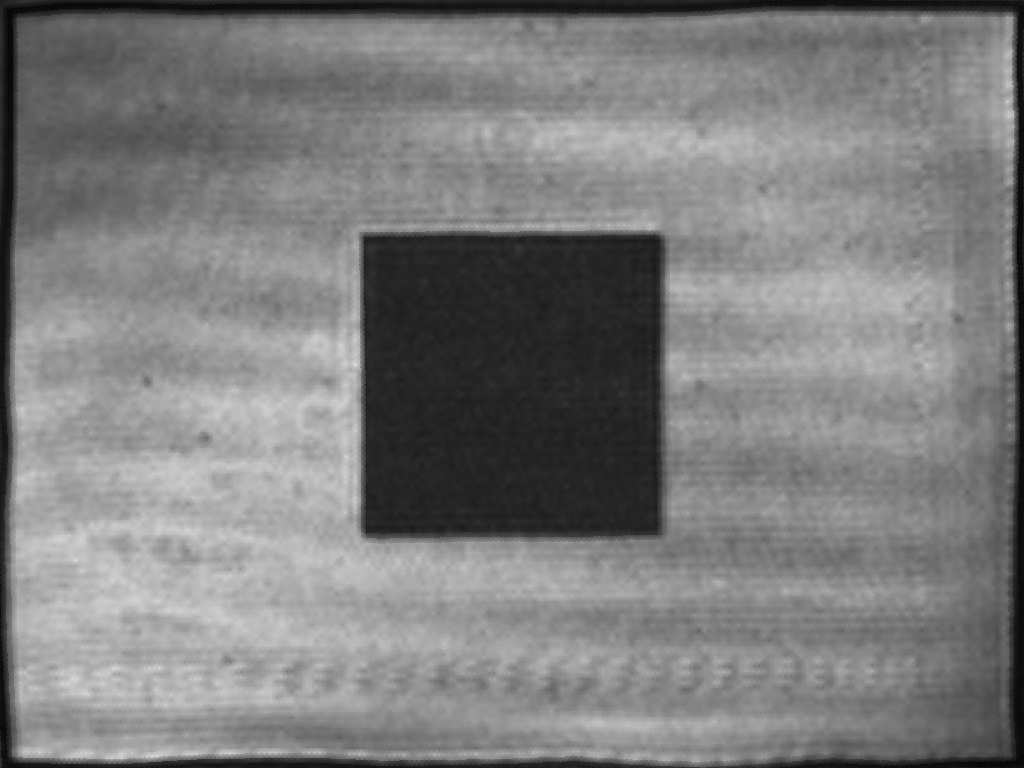
\includegraphics[width=\linewidth]{DMD/Results/EdgeExamples/05}
        \caption{Detection radius: \SI{5}{px}}
    \end{subfigure}
    \begin{subfigure}[t]{0.43\textwidth}
        \centering
        
\includegraphics[width=\linewidth]{DMD/Results/EdgeExamples/15}
        \caption{Detection radius: \SI{15}{px}}
    \end{subfigure}
    \caption[Influence of the edge detection radius on the overcorrection of the intensity in the centre]{Influence of the edge detection radius on the overcorrection of the intensity in the centre. The contrast in (a) is much lower than in (b).}
    \label{fig:edge_detection_test_example}
\end{figure}
\iffalse
\section{Spots of Varying Brightness}
The next test is performed by adding gaussian peaks with varying intensity as deviations. This leads to a final image that should contain a flat plateau with a gaussian indentation in the centre. This is portrayed in Figure~\ref{fig:dmd_results_gaussian_example}. 
\begin{figure}[htbp]
    \centering
    \begin{subfigure}[c]{0.43\textwidth}
        \centering
        \frame{
\includegraphics[width=\linewidth]{DMD/Results/square-target}}
        \caption{Target}
    \end{subfigure}
    \begin{subfigure}[c]{0.43\textwidth}
        \centering
        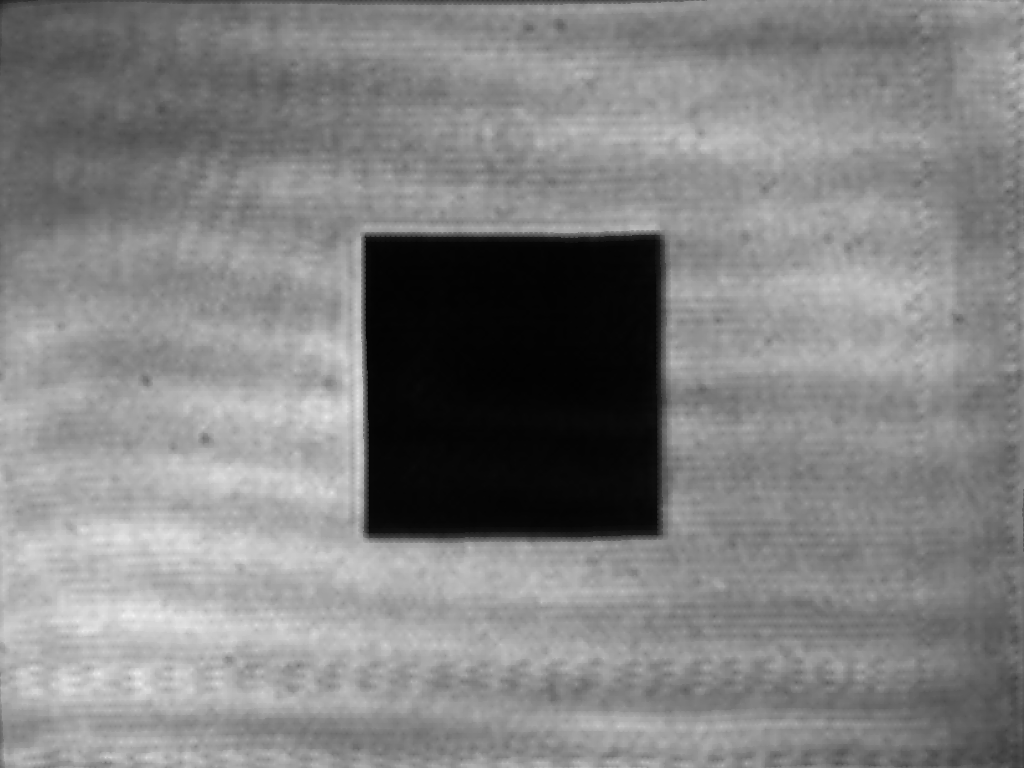
\includegraphics[width=\linewidth]{DMD/Results/GaussianExamples/090-orig}
        \caption{Original camera image}
    \end{subfigure} \\
    \begin{subfigure}[c]{0.43\textwidth}
        \centering
        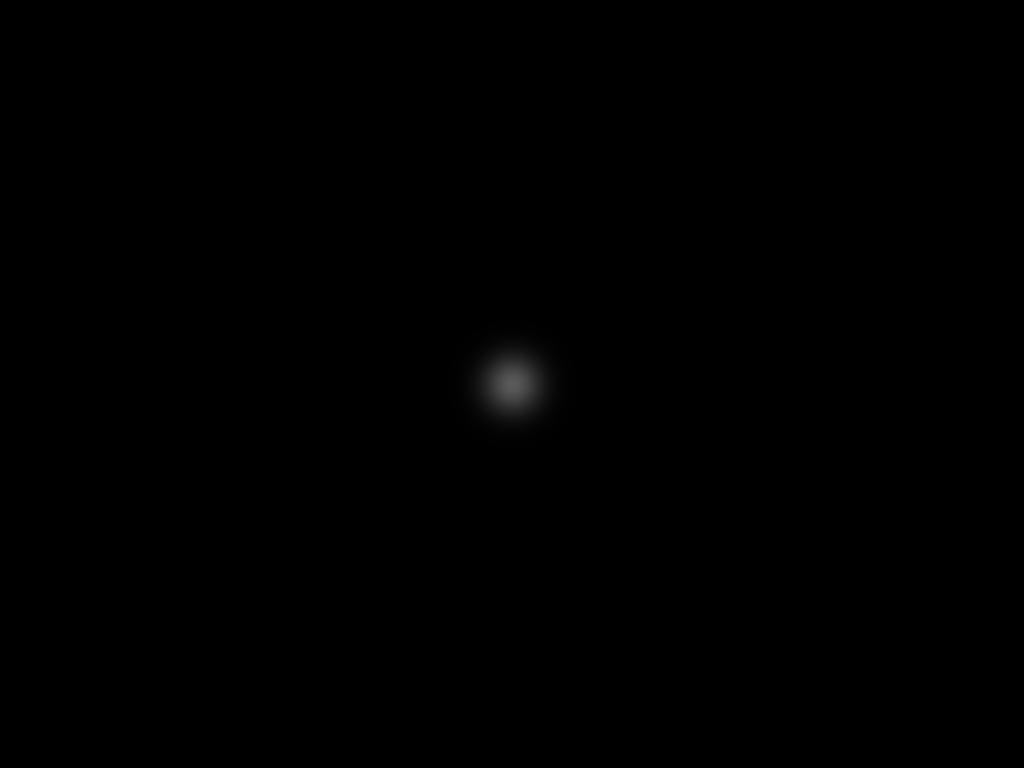
\includegraphics[width=\linewidth]{DMD/Results/GaussianExamples/090-offs}
        \caption{Added deviation}
    \end{subfigure}
    \begin{subfigure}[c]{0.43\textwidth}
        \centering
        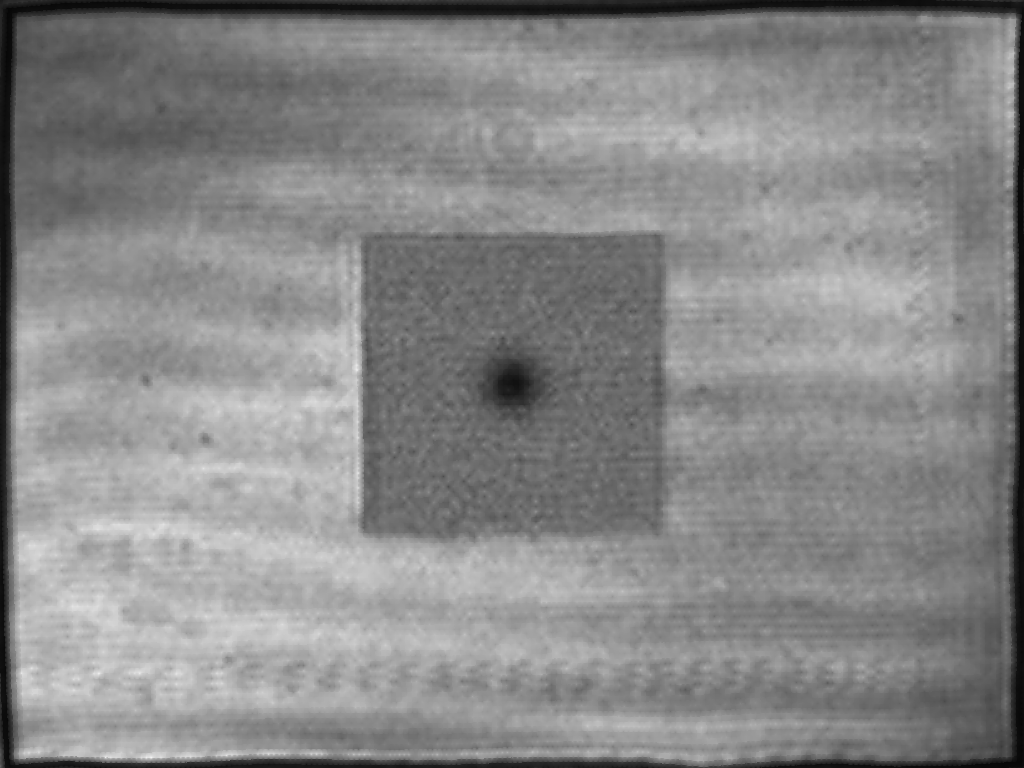
\includegraphics[width=\linewidth]{DMD/Results/GaussianExamples/090-final}
        \caption{Corrected image}
    \end{subfigure}
    \caption[Test example with added gaussian peak]{Test example with added gaussian peak. The positive deviation (c) resutls in an indentation in the corrected image (d).}
    \label{fig:dmd_results_gaussian_example}
\end{figure}
We can fit a 2D gaussian profile to this to determine how well the artificial deviation has been corrected. The added intensity is of the form
\begin{align*}
    I_\text{error} &= A_0\cdot\exp\!\left(-\frac{x^2+y^2}{2\sigma_0^2}\right), \ \sigma_0 = \SI{20}{px}
    \intertext{and correspondingly, the fitted intensity to the corrected picture is}
    I_\text{fit} &= C - A\cdot\exp\!\left(-\frac{(x-\mu_x)^2+(y-\mu_y)^2}{2\sigma^2}\right)
\end{align*}
We measure the goodness of the correction by looking at the relative difference between original gaussian amplitude $A_0$ and the amplitude of the indentation $A$ (Fig.~\ref{fig:dmd_results_gaussian_peak})
% as well as the difference between the corrected mean intensity $C$ and $A_0$ (Fig.~\ref{fig:dmd_results_gaussian_plateau}). The latter gives an indication as to how far the overall intensity has been over- or undercorrected
. 
A plot with horizontal cuts through the central region of the images is also shown in Figure~\ref{fig:dmd_results_gaussian_cuts}.
\begin{figure}[htbp]
    \centering
    \includegraphics[]{DMD/Results/IntensityCorrPeak}
    \caption[Difference between peak height in added deviation and in corrected image]{Difference between peak height in added deviation and in corrected image. Errorbars show the fitting erros.}
    \label{fig:dmd_results_gaussian_peak}
\end{figure}
\todo[inline]{FINDE IRGENDEINE VERFICKTE BEGRÜNDUNG WARUM DER SCHEISS SO SCHEISSE IST WIE ER IST}
% \begin{figure}[htbp]
%     \centering
%     \includegraphics[]{DMD/Results/IntensityCorrAvg}
%     \caption[Difference between Plateau Intensity and Added Peak Height]{Difference between Plateau Intensity and Added Peak Height. Errorbars show fitting errors and are to small to be visible.}
%     \label{fig:dmd_results_gaussian_plateau}
% \end{figure}
\fi % IF THIS IS PUT BACK IN, ALSO PUT THE CUTS BACK INTO THE APPENDIX

\section{Resolution}
Next, we want to see how great the resolving power of the algorithm is. We add artifical deviations that contain sinusoidal wave patterns with varying periods to the camera image (see Fig.~\ref{fig:dmd_results_resolution_example}).
\begin{figure}[htbp]
    \centering
    \begin{subfigure}[c]{0.43\textwidth}
        \centering
        \frame{
\includegraphics[width=\linewidth]{DMD/Results/square-target}}
        \caption{Target}
    \end{subfigure}
    \begin{subfigure}[c]{0.43\textwidth}
        \centering
        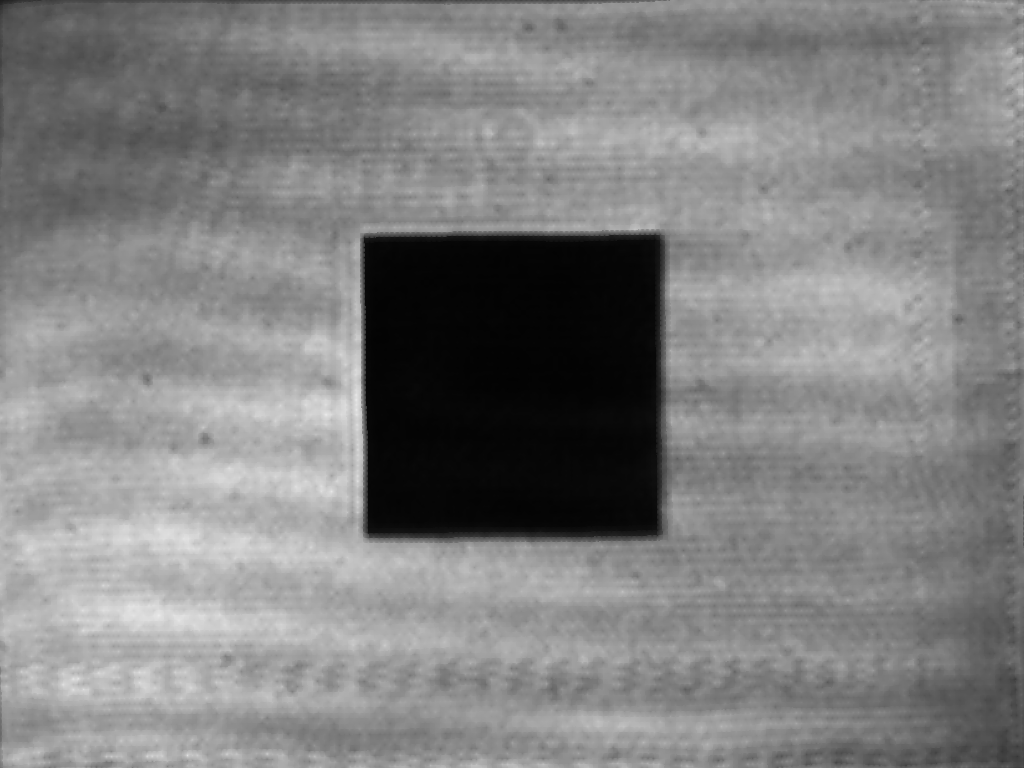
\includegraphics[width=\linewidth]{DMD/Results/ResolutionExamples/15-orig}
        \caption{Original camera image}
    \end{subfigure}
    \begin{subfigure}[c]{0.43\textwidth}
        \centering
        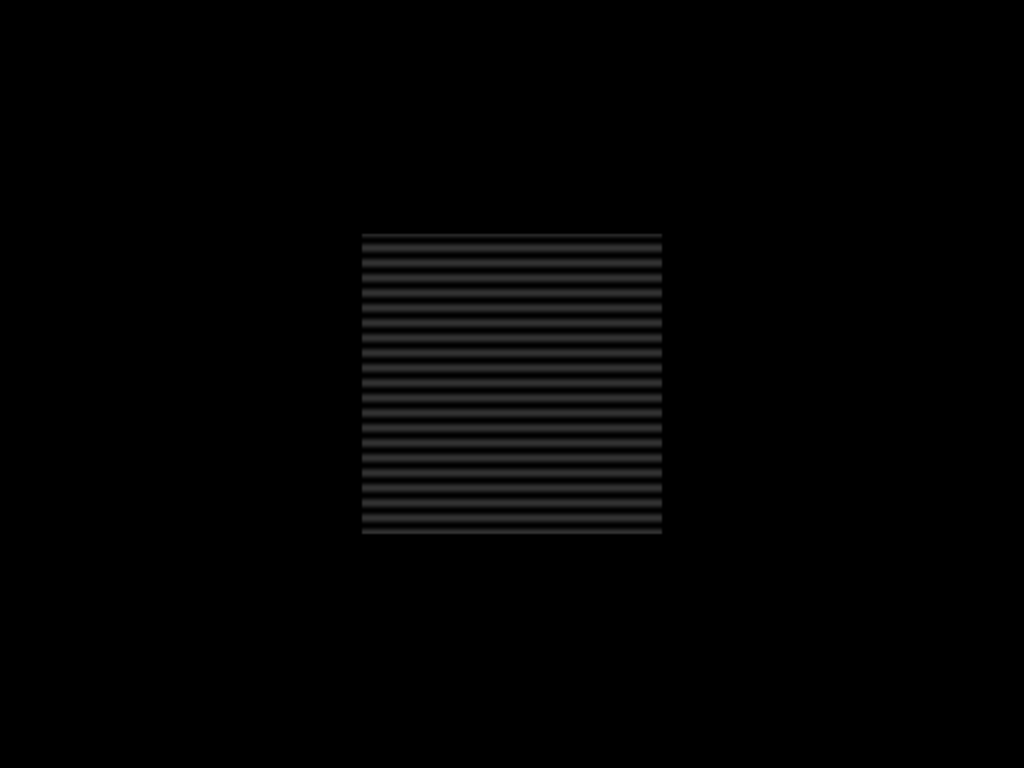
\includegraphics[width=\linewidth]{DMD/Results/ResolutionExamples/15-offs}
        \caption{Added deviation}
    \end{subfigure}
    \begin{subfigure}[c]{0.43\textwidth}
        \centering
        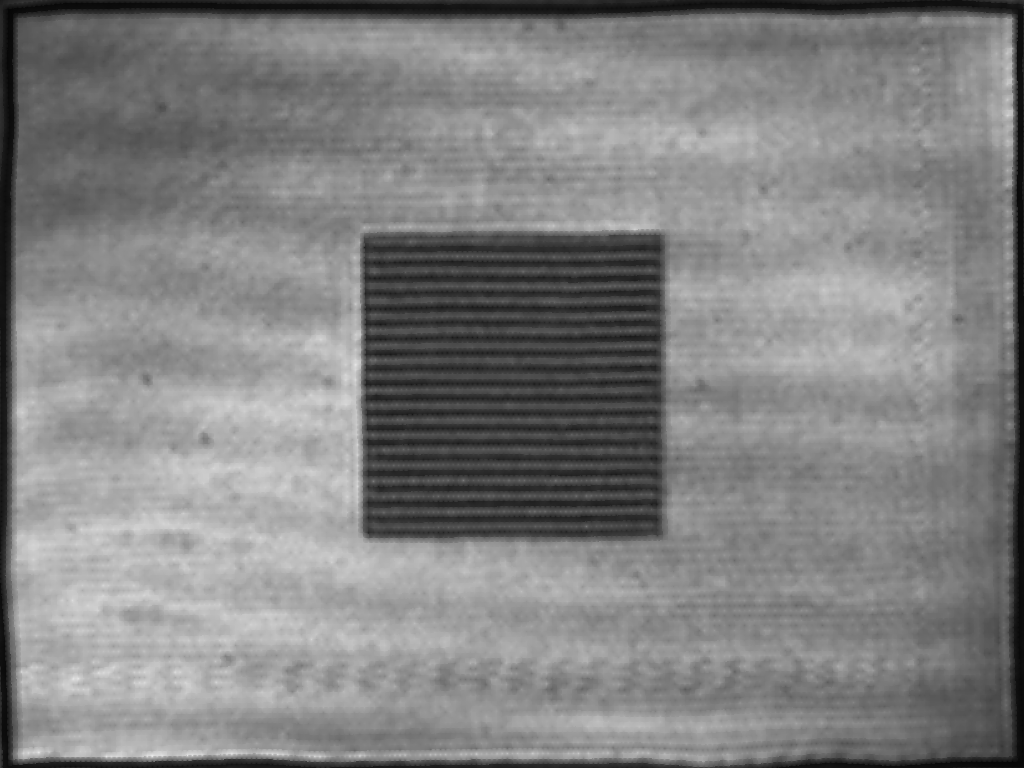
\includegraphics[width=\linewidth]{DMD/Results/ResolutionExamples/15-final}
        \caption{Corrected image}
    \end{subfigure}
    \caption[Test example with added wave pattern]{Test example with added wave pattern. The pattern seen in (c) appears inverted in the corrected image (d) which can be seen from the shift of the intensity maxima.}
    \label{fig:dmd_results_resolution_example}
\end{figure}
The result can then be analysed if the modulation could be resolved. The central square is averaged in the horizontal direction and a wave pattern is then fitted to the result.
\begin{align}
    I_\text{error} &=  A_0 \cdot \frac{1-\cos(2\pi y / \lambda_0)}{2},\ A_0 = 50 \\
    I_\text{fit}   &= C + A \cdot \frac{1 - \cos(2\pi (y-\varphi) / \lambda)}{2}
\end{align}
The findings for $A(\lambda_0)$ are shown in Figure~\ref{fig:dmd_results_resolution_amplitude} and the fits for the 5:1 magnification are displayed in Figure~\ref{fig:dmd_results_resolution_cuts}.
\begin{figure}[htbp]
    \centering
    \includegraphics[]{DMD/Results/LengthScaleAmp}
    \caption[Detected amplitude of the wave pattern depending on the period]{Detected amplitude of the wave pattern depending on the period. The solid lines are errorfunction fits (Eq.~\eqref{eq:errorfunction}, results in Tab.~\ref{tab:dmd_resolution_fits}). Except for the first datapoint of the lower magnification, the errorbars are too small to be visible. The dotted orange line is a continuation of the fitted function for this magnification over the rest of the data range.}
    \label{fig:dmd_results_resolution_amplitude}
\end{figure}
For low spacing between the fringes, the pattern cannot be resolved but after a threshold period $\lambda_\text{threshold}$ is reached, the full amplitude $A_0$ can be reproduced in the corrected image. To determine this threshold, we fit the function 
\begin{equation}
    A(\lambda_0) = \tilde{A}\left[ 1 + \text{erf}\!\left(\frac{\lambda_0 - \lambda_\text{threshold}}{\sigma}\right) \right] \label{eq:errorfunction}
\end{equation}
to the data, the results of which are summarised in Table~\ref{tab:dmd_resolution_fits}.
\begin{table}[htbp]
    \centering
    \begin{tabular}{S[table-format=1.1]S[table-format=2.2(2)]S[table-format=2.2(2)]S[table-format=1.2(2)]}
        \toprule
        \multicolumn{1}{c}{Magnification} & \multicolumn{1}{c}{$\tilde{A}$} & \multicolumn{1}{c}{$\lambda_\text{threshold}$} & \multicolumn{1}{c}{$\sigma$} \\
        \midrule
        2.2 & 53.11+-0.64 & 6.71+-0.18 & 1.07+-0.21 \\
        5   & 50.37+-0.22 & 13.49+-0.08 & 2.48+-0.15 \\
        \bottomrule
    \end{tabular}
    \caption{Results of the fits in Fig.~\ref{fig:dmd_results_resolution_amplitude}}
    \label{tab:dmd_resolution_fits}
\end{table}
If we divide the threshold period by the magnification, we see that $\sim\!\SI{3}{px}$ are necessary on the camera to resolve two lines. This is a great result because with the \SI{1}{px} blur of the camera image taken into account, this is very close to the \enquote{perfect} result of \SI{2}{px}.

\pagebreak
\section{Randomised Noisefloor}
The last test is to add a random noise pattern with different levels of fluctuation as a deviation to the camera image. After the algorithm has converged, this noise pattern should appear as a negative in the camera image. We then add the same noise pattern back on top, which would yield an image with no remaining fluctuations in case the algorithm works perfectly. Thus, evaluating the remaining RMS error (over the central $300\times \SI{300}{px}$ square) is a measure of the correction quality. We have already established in the previous step that the patches need to have a certain separation to be resolvable. It is therefore not as straightforward as using a noisy image with individual randomised pixel intensities. In this test, we create noise of a certain height $H$ by distributing random intensities from a gaussian distribution with mean $H$ and standard deviation $H$ over a rectangle with half the side lengths of the DMD. Intensities lower than 0 are cut off. The complete pattern is then blurred with a radius of \SI{7}{px} and scaled up to the full size of the DMD. This ensures that the noise pattern can be resolved by the correction algorithm. An example of a noise pattern generated this way is shown in Figure~\ref{fig:dmd_noise_example}.
\begin{figure}[htbp]
    \centering
    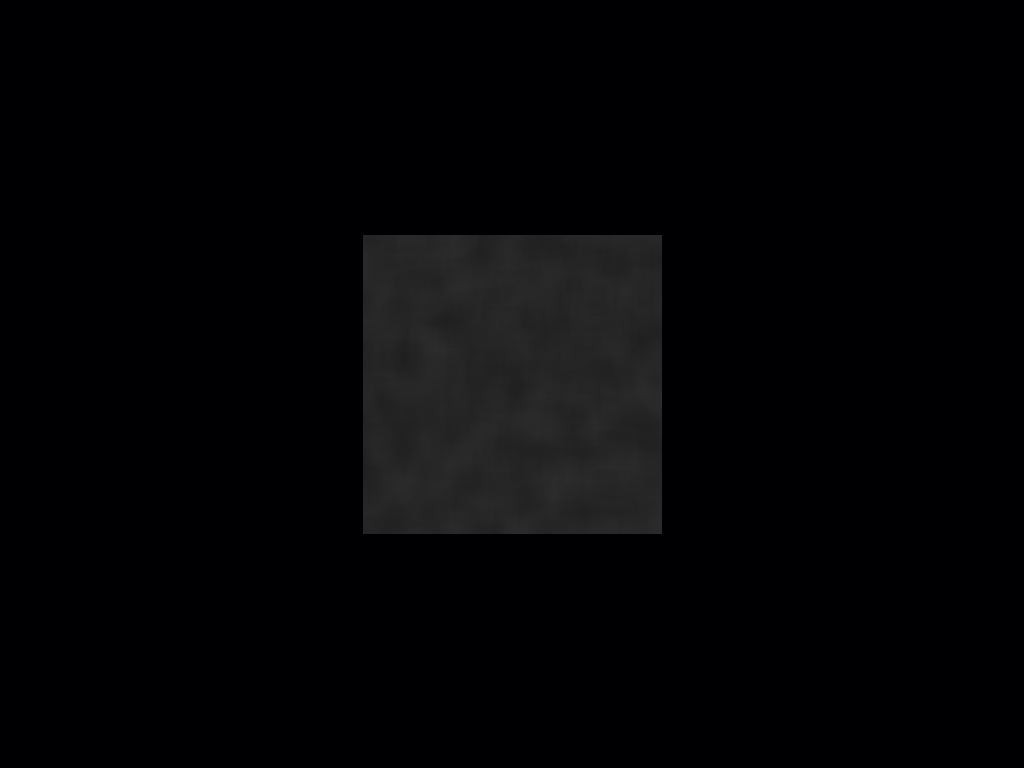
\includegraphics[width=.43\textwidth]{DMD/Results/NoiseExamples/35}
    \caption{Artificial noise pattern generated with a height of $H=35$}
    \label{fig:dmd_noise_example}
\end{figure}
To get statistically significant results, we run the test 100 times for each height $H$ and each magnification.
%
Table~\ref{tab:dmd_noise_results} shows the averages for the initial RMS error of the noise pattern $\Delta_0$, the final RMS error after convergence is reached $\Delta_\text{final}$ and number of iterations necessary $N$. 
\begin{table}[htbp]
    \centering
    \begin{tabular}{S[table-format=1.1]S[table-format=2]S[table-format=2.2(1)]S[table-format=2.2(1)]S[table-format=2.1(2),separate-uncertainty=true]}
        \toprule
        \multicolumn{1}{c}{Magnification} & \multicolumn{1}{c}{Height $H$} & \multicolumn{1}{c}{$\Delta_0$ / \si{\percent}} & \multicolumn{1}{c}{$\Delta_\text{final}$ / \si{\percent}} & \multicolumn{1}{c}{$N$} \\
        \midrule
        {\multirow{4}{*}{$\num{2.2}$}} & 5 & 2.07 +- 0.01 & 0.68 +- 0.03 & 8.3 +- 0.9 \\
        & 15 & 6.28 +- 0.03 & 0.74 +- 0.03 & 8.8 +- 1.2 \\
        & 25 & 10.48 +- 0.06 & 0.78 +- 0.03 & 8.6 +- 1.1 \\
        & 35 & 14.68 +- 0.09 & 0.88 +- 0.04 & 8.2 +- 1.2 \\
        \midrule
        {\multirow{4}{*}{$5\negphantom{5}\phantom{\num{2.2}}$}} & 5 & 2.07 +- 0.01 & 0.56 +- 0.03 & 9.9 +- 1 \\
        & 15 & 6.28 +- 0.03 & 0.64 +- 0.04 & 9.1 +- 0.9 \\
        & 25 & 10.48 +- 0.06 & 0.75 +- 0.05 & 8.5 +- 1.3 \\
        & 35 & 14.68 +- 0.09 & 0.82 +- 0.05 & 9.2 +- 1.4 \\
        \bottomrule
    \end{tabular}
    \caption{Summarised results from the noise pattern corrections}
    \label{tab:dmd_noise_results}
\end{table}
In all cases, the final RMS error is below \SI{1}{\percent} and in most cases, less than 12 iterations were necessary to reach this error. With increasing noisefloor height, a larger portion of the DMDs dynamic range can be utilised for the correction, giving a larger improvement relative to the initial error. 
%
Finally, we show the evolution of the deviation relative to $\Delta_0$ over the first $\tilde{N} = \mu_N + \sigma_N$ iterations (average $+$ one standard deviation, see Table~\ref{tab:dmd_noise_results}) in Figure~\ref{fig:dmd_results_noise_evolution}. The reason that the relative error starts above $1$ in some cases is that the edge detection radius was not high enough, meaning that the maximum deviation detected at the edges of the square were greater than from the noise pattern.
\begin{figure}[h!tbp]
    \centering
    \includegraphics[]{DMD/Results/IterationsErrorEvo}
    \caption[Error evolution in the correction of a randomised noise pattern]{Error evolution in the correction of a randomised noise pattern. Errorbars are omitted because they were too small to be visible.}
    \label{fig:dmd_results_noise_evolution}
\end{figure}


% This is an excellent result and strongly indicates that this method can indeed be used to correct for additional light that does not come from the DMD itself.

% \begin{figure}[htbp]
%     \centering
%     \includegraphics[]{DMD/Results/IterationsFinalError}
%     \caption{COOL CAPTION GOES HERE}
%     \label{fig:dmd_results_noise_finalerror}
% \end{figure}
% \begin{figure}[htbp]
%     \centering
%     \includegraphics[]{DMD/Results/IterationsNumber}
%     \caption{COOL CAPTION GOES HERE}
%     \label{fig:dmd_results_noise_number}
% \end{figure}
